\section{Attachements}
\subsection{A1 Tiefpassentwurf mit fir()}
Mit der Matlab Funktion fir() ist ein FIR-Tiefpassfilter zu entwerfen. Um die geforderten Grenzwerte einzuhalten muss zunächst die Filterordnung mit dem M\_File Kaiser\_Order\_01.m bestimmt werden. Die Koeffizienten werden mit dem M\_File fir\_1.m gemäß Listing 2 bestimmt. Außerdem wird der Amplitudengang (x=normiert auf Fs/2), das Zeitsignal und der Frequenzgang vor sowie nach dem Filter in einem Diagramm ausgegeben. Die normierten Filterkoeffizienten (normiert auf $\pm$ 1) müssen für die spätere Implementierung in den DSP auf 16-Bit Integer werte angepasst werden. Dazu werden die Koeffizienten mit einem Korrekturfaktor versehen. In Abbildung \ref{lst:fir_2a_matlab} sind die Änderungen von Listing 2 aufgeführt.\\Korrekturwert maximal 1 $\approx$ 32767 $\rightarrow$ 1-Bit Vorzeichen + 15-Bit Wertebereich.

\begin{equation}
b_{k}(x) = b(x) * 2^{15}-1
\end{equation}

\begin{table}[h]
	\centering
	\begin{tabular}{c | c}
		Parameter	& Wert	\\
		\hline
		Eckfrequenz Durchlassbereich			& $1800~Hz$	\\
		Eckfrequenz Sperrbereich				& $2600~Hz$	\\
		Maximaler Ripple im Durchlassbereich	& $0.5~db$	\\
		Minimale Sperrdämpfung					& $40~db$	\\
		Abtastfrequenz							& $8000~Hz$	\\
	\end{tabular}
\end{table}

\lstinputlisting[style=matlab, caption={fir\_2a.m Matlab-File Auszug - Tiefpassfilter Ordnung 23}, label={lst:fir_2a_matlab}]{Code/fir_2a.m}

\newpage

\lstinputlisting[style=c, caption={FIR-Filter Koeffizienten Ordnung 23}, label={lst:fir_2a_koeff}]{Code/LP_coeff.h}

\begin{figure}[h]
\centering
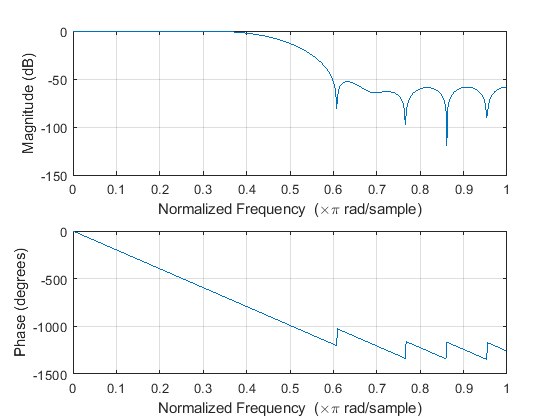
\includegraphics[width=0.8\linewidth]{Bilder/Attachment_A1_fir_2a_Amplitudengang}
\caption{Amplituden und Phasengang - FIR-Filter Tiefpass}
\label{fig:Attachment_A1_fir_2a_Amplitudengang}
\end{figure}

\newpage

\begin{figure}[h]
\centering
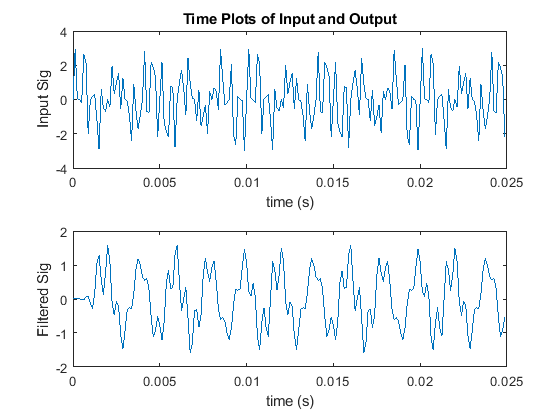
\includegraphics[width=0.6\linewidth]{Bilder/Attachment_A1_fir_2a_Timeplot}
\caption{Eingangs- und gefiltertes Ausgangszeitsignal  - FIR-Filter Tiefpass}
\label{fig:Attachment_A1_fir_2a_Timeplot}
\vspace{-10pt}
\end{figure}

\begin{figure}[h]
\centering
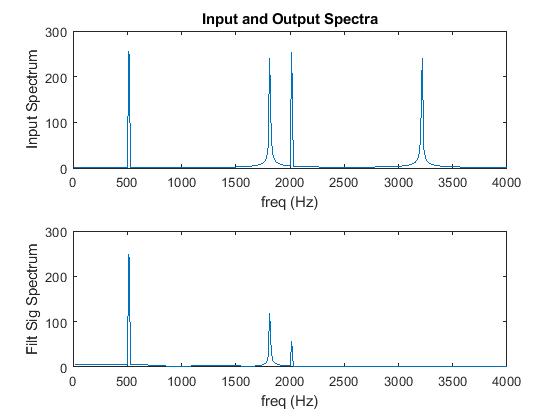
\includegraphics[width=0.6\linewidth]{Bilder/Attachment_A1_fir_2a_Spektrum}
\caption{Eingangs- gefiltertes Ausgangs Frequenzspektrum}
\label{fig:Attachment_A1_fir_2a_Spektrum}
\end{figure}

\newpage

\subsection{A2 Tiefpassentwurf mit firpm()}

\lstinputlisting[style=matlab, caption={fir\_2b.m Matlab-File Auszug - Tiefpassfilter Ordnung 16}, label={lst:fir_2b_matlab}]{Code/fir_2b.m}

\lstinputlisting[style=c, caption={FIR-Filter Koeffizienten Ordnung 16}, label={lst:fir_2b_koeff}]{Code/LP_coeff_firpm.h}

\clearpage

\begin{figure}[h]
\centering
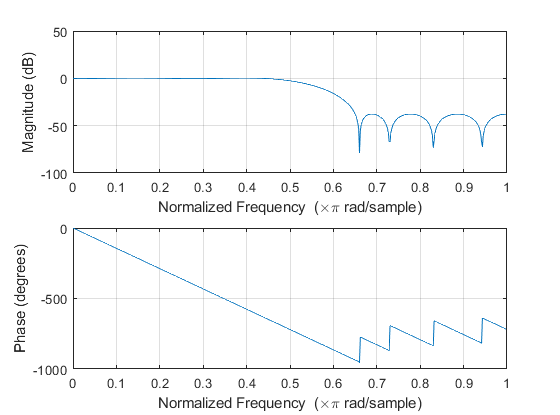
\includegraphics[width=0.7\linewidth]{./Bilder/Attachment_A2_fir_2b_Amplitudengang}
\caption{Amplituden und Phasengang - FIR-Filter Tiefpass}
\label{fig:Attachment_A2_fir_2b_Amplitudengang}
\vspace*{30mm}
\centering
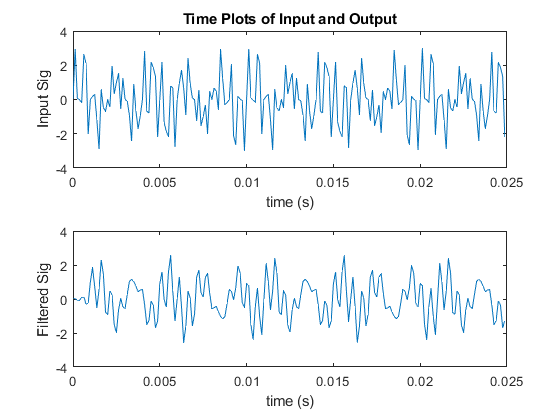
\includegraphics[width=0.7\linewidth]{./Bilder/Attachment_A2_fir_2b_Timeplot}
\caption{Eingangs- und gefiltertes Ausgangszeitsignal  - FIR-Filter Tiefpass}
\label{fig:Attachment_A2_fir_2b_Timeplot}
\end{figure}

\clearpage

\begin{figure}[h]
\centering
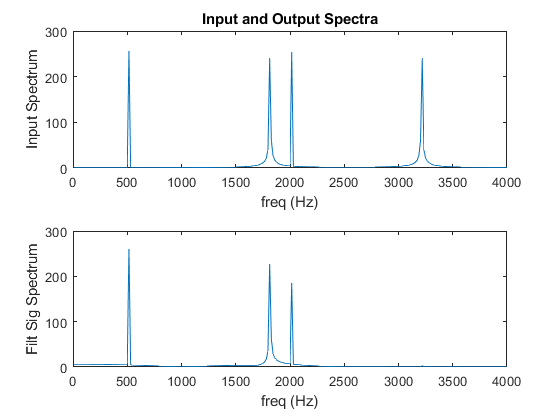
\includegraphics[width=0.7\linewidth]{./Bilder/Attachment_A2_fir_2b_Spektrum}
\caption{Eingangs- gefiltertes Ausgangs Frequenzspektrum}
\label{fig:Attachment_A2_fir_2b_Spektrum}
\end{figure}


\clearpage

\subsection{B Bandpass-Filterentwurf}

\lstinputlisting[style=matlab, caption={fir\_3.m Matlab-File Auszug - Bandpassfilter Ordnung 45}, label={lst:fir_3_matlab}]{Code/fir_3.m}

\lstinputlisting[style=c, caption={FIR-Filter Koeffizienten Ordnung 45}, label={lst:fir_3_koeff}]{Code/BP_coeff.h}

\begin{figure}[h]
\centering
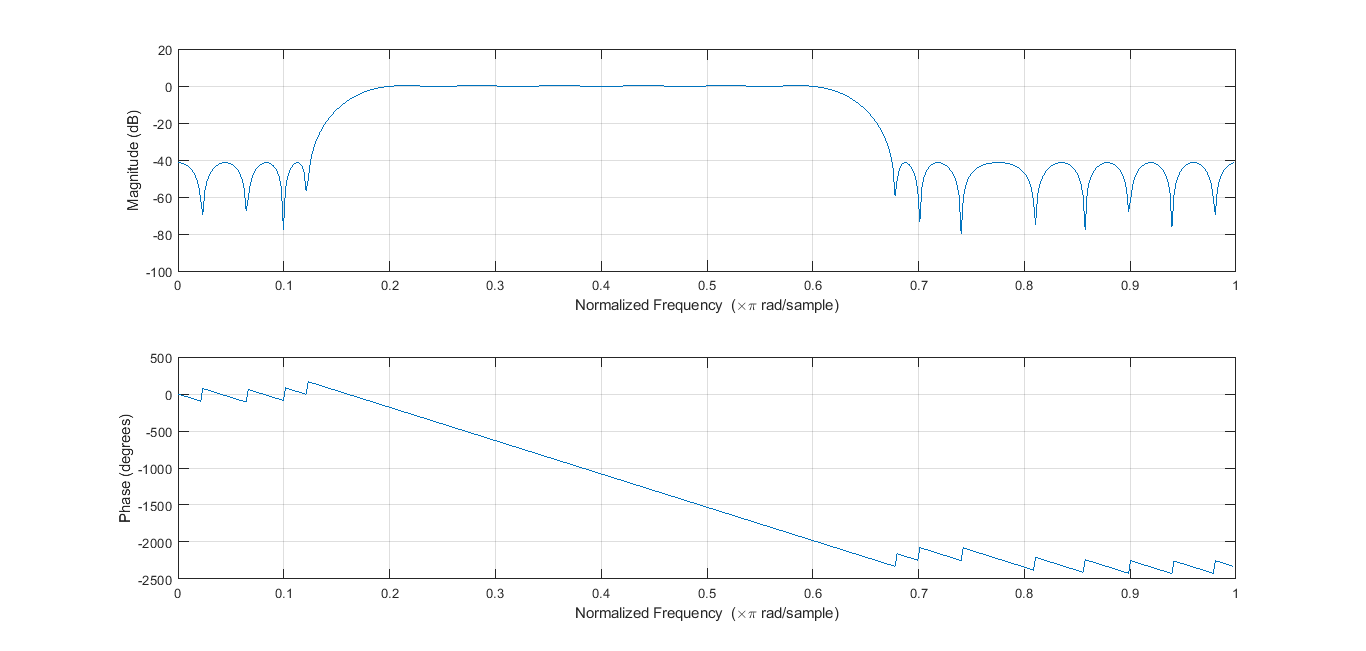
\includegraphics[width=0.7\linewidth]{./Bilder/Attachment_B_fir_3_Amplitudengang}
\caption{Amplituden und Phasengang - FIR-Filter Bandpass}
\label{fig:Attachment_B_fir_3_Amplitudengang}
\end{figure}

\begin{figure}[h]
\centering
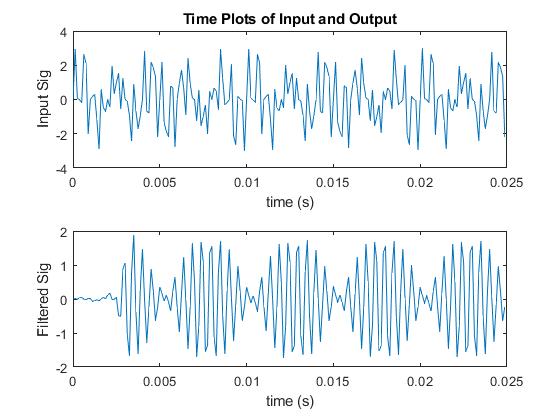
\includegraphics[width=0.7\linewidth]{./Bilder/Attachment_B_fir_3_Timeplot}
\caption{Eingangs- und gefiltertes Ausgangszeitsignal  - FIR-Filter Bandpass}
\label{fig:Attachment_B_fir_3_Timeplot}
\end{figure}

\clearpage

\begin{figure}[h]
\centering
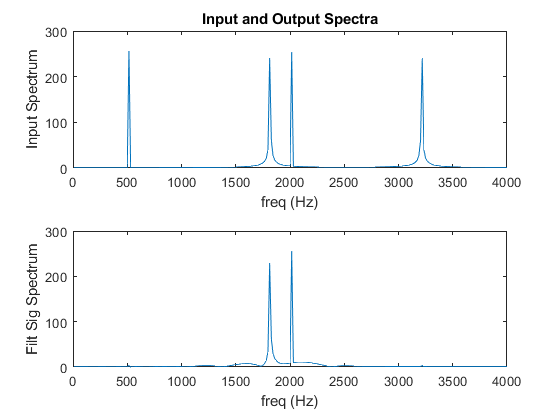
\includegraphics[width=0.7\linewidth]{./Bilder/Attachment_B_fir_3_Spektrum}
\caption{Eingangs- gefiltertes Ausgangs Frequenzspektrum}
\label{fig:Attachment_B_fir_3_Spektrum}
\end{figure}

\clearpage

\subsection{C1 Analoge Übertragungscharakteristik des DSK Boards}
\noindent Zu Beginn dieses Laborversuchs wurde ein Projekt zu Eingabe sowie anschließenden Ausgabe dieser eingelesenen Werte realisiert, um den Frequenzgang des DSK-Boards zu bestimmen. Im UVP Analyzer wurde ein Messung mit Frequenzsweep bis 8kHz durchgeführt.

\begin{figure}[h]
	\centering
	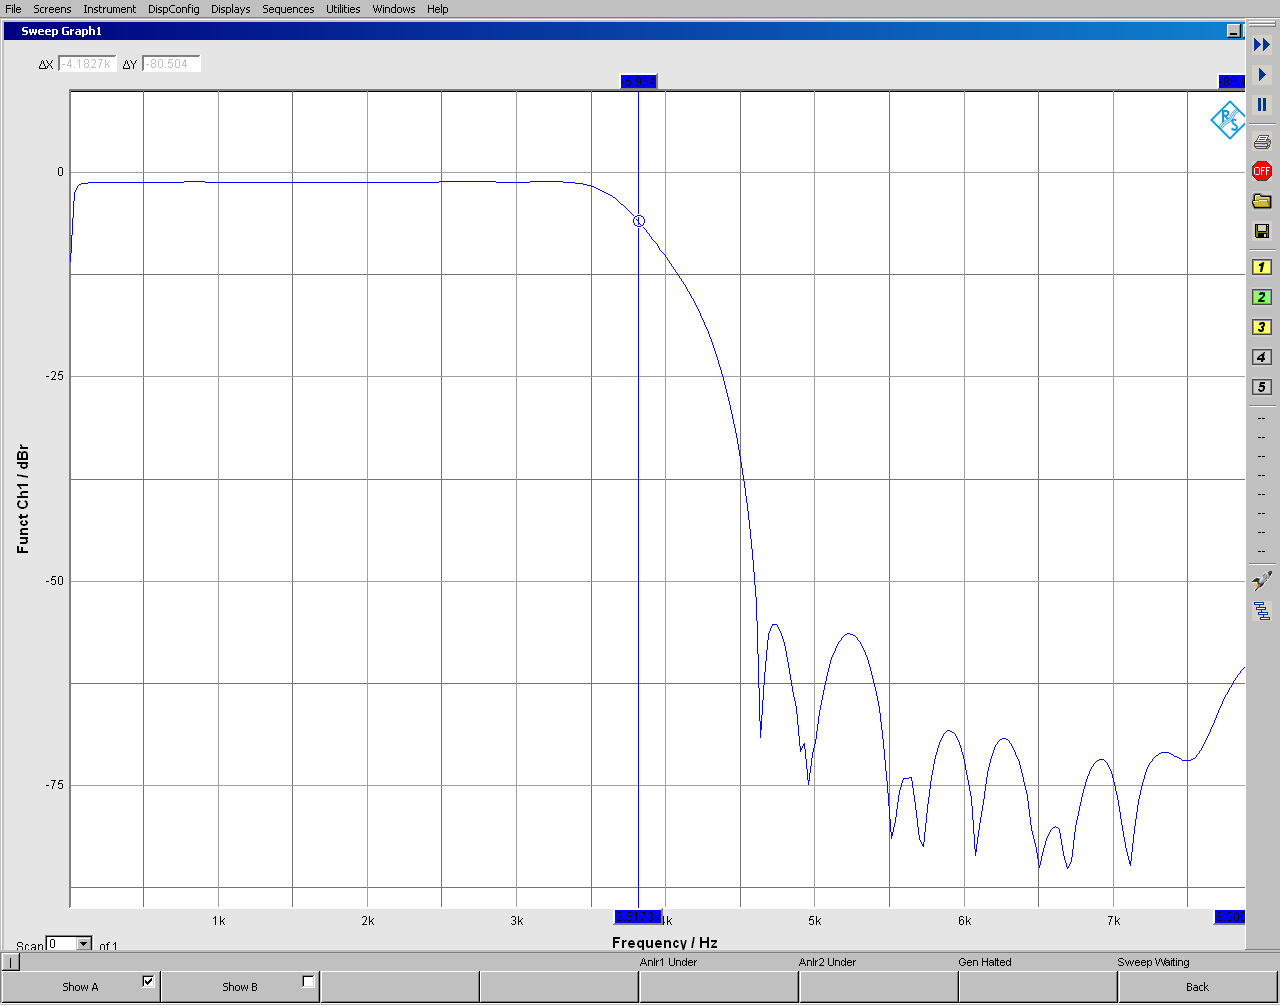
\includegraphics[width=1\linewidth]{Bilder/Attachment_C1_DSK_Frequenzgang}
	\caption{Frequenzgang des DSK-Boards}
	\label{fig:Attachment_C1_DSK_Frequenzgang}
\end{figure}

\noindent Wir können ganz klar Tiefpassverhalten des DSK-Boards erkennen. Dies ist für die nächsten Messungen zu berücksichtigen.

\clearpage

\subsection{C2 Echtzeit-Festkomma-Impementierung des FIR-Filters}
\noindent Alle Projekteinstellungen sowie -konfigurationen wurden nach Laboranleitung durchgeführt.\\
\noindent Folgende Änderungen wurden durch uns in fir\_a.c ergänzt: \\
\lstinputlisting[style=c, caption={fir\_a.c C-File Auszug - ISR Tiefpass FIR}, label={lst:fir_a_ISRTP}]{Code/fir_a.c}
\noindent Diese Implementierung in der for-Schleife ab Zeile 18 sowie die anschließende Überschreibung des Wertes (32 Bit auf 16 Bit) nach Beendigung der for-Schleife ist vorteilhaft bezüglich des Rauschverhaltens/der Genauigkeit, da in der erwähnten for-Schleife mit 32 Bit zugunsten der Genauigkeit gerechnet wird. Hierbei treten nur sehr geringe Rundungsfehler auf. Dieser Wert wird dann erst nach der Berechnung auf 16 Bit gecastet. Somit rechnet man so lange wie möglich mit einer hohen Genauigkeit, ohne allzu große Rundungsfehler zu produzieren.

\clearpage

\begin{figure}[h]
	\centering
	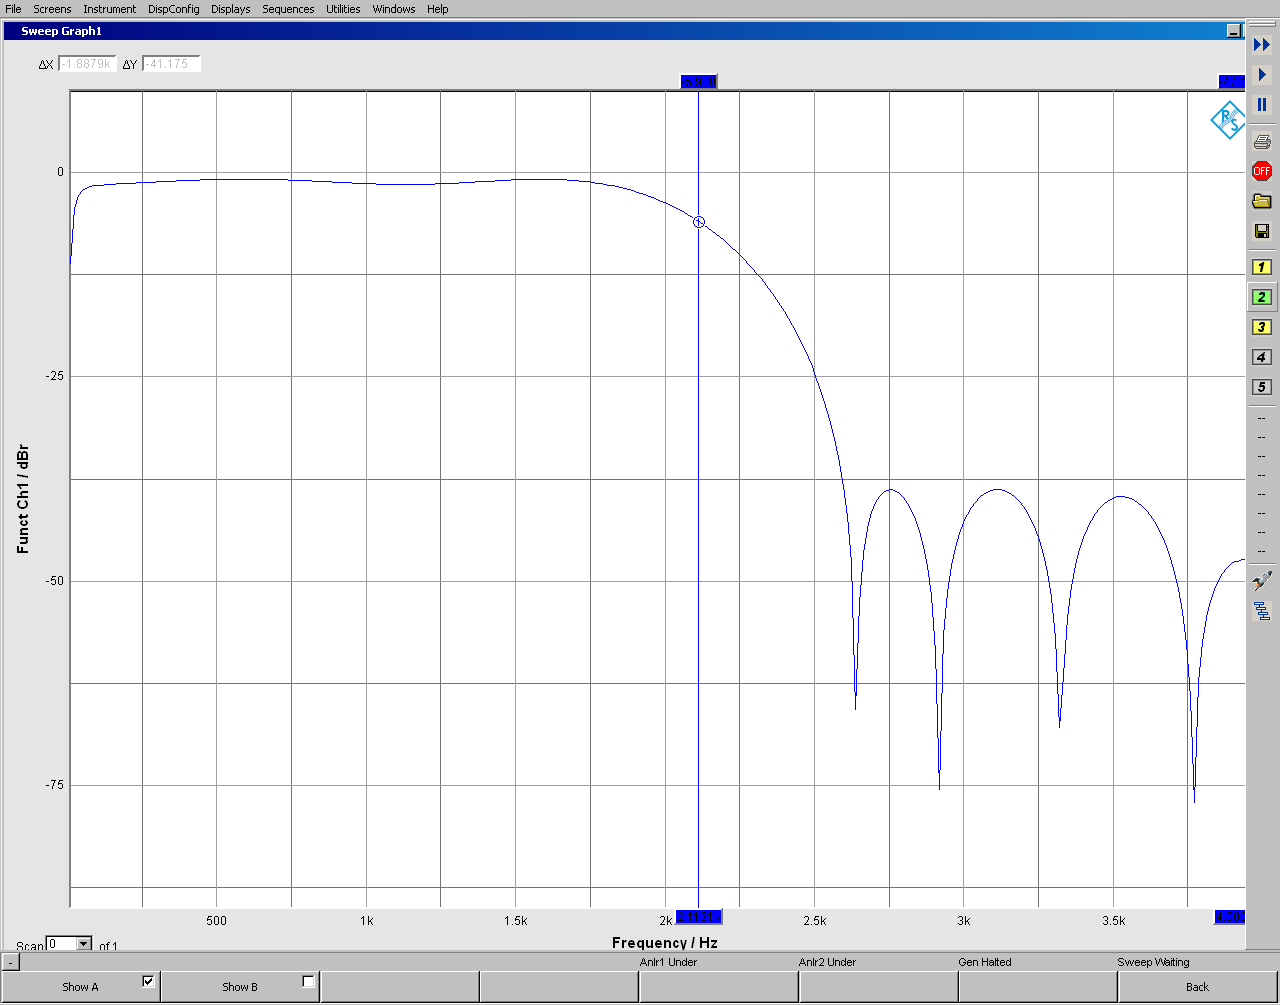
\includegraphics[width=1\linewidth]{Bilder/Attachment_C2_TP_Fg}
	\caption{Messung: Frequenzgang des Tiefpasses mit einem 4kHz Frequenzsweep}
	\label{fig:Attachment_C2_TP_Fg}
\end{figure}

\subsection{C3 Vergleich des Amplitudenganges vom FIR-Filter Matlab - DSK Board}
\noindent Bei der Beurteilung des Amplitudenganges des FIR-Filters muss stets ebenso der Amplitudengang des DSK-Boards berücksichtigt werden. Wie auf Abbildung \ref{fig:Attachment_C1_DSK_Frequenzgang} zu sehen, werden Frequenzen ab 3.5 kHz erst wenig, dann ab $f_g \approx 3.85kHz$) aufgrund des vorgeschalteten Tiefpassfilters (Anti-Aliasingfilter) stärker gedämpft. Mit Berücksichtigung dieser Information fällt beim Frequenzgang des FIR-TP-Filter (Abb. \ref{fig:Attachment_C2_TP_Fg}) auf, dass die letzte Nebenkeule stärker gedämpft wird als die restlichen vorangegangen Nebenkeulen. Dies geschieht, da bei einer Startfrequenz von $\approx3.8kHz$ der letzten sichtbaren Nebenkeule das Anti-Aliasingfilter des DSK-Boards einen entscheidenden  Einfluss bekommt. Dieses Eingangsfilter dämpft bei dieser Frequenz von $\approx3.8kHz$ bereits um fast 6dB. Die Frequenzen $<3.8kHz$ befinden sich im Durchgangsbereich des Eingangsfilters. Diese ermittelte Grenzfrequenz ist durch die Wahl unserer internen Abtastfrequenz von 8kHz bedingt.

\clearpage

\subsection{D Profiling FIR-ISR}
\noindent Ein Profiling der FIR-ISR wurde durchgeführt. Hierbei wurden die vergangen Takte gezählt die benötigt werden, um die ISR vom Eintreten bis zur Beendigung dieser durchzulaufen. Der Inhalt der ISR war bei dieser Messung in die Main (vor Freigabe jeglicher Interrupts) einzufügen. Es wurden eine Anzahl von 1359 Takten bei einer Taktfrequenz von 225Mhz gemessen.

\begin{figure}[h]
	\centering
	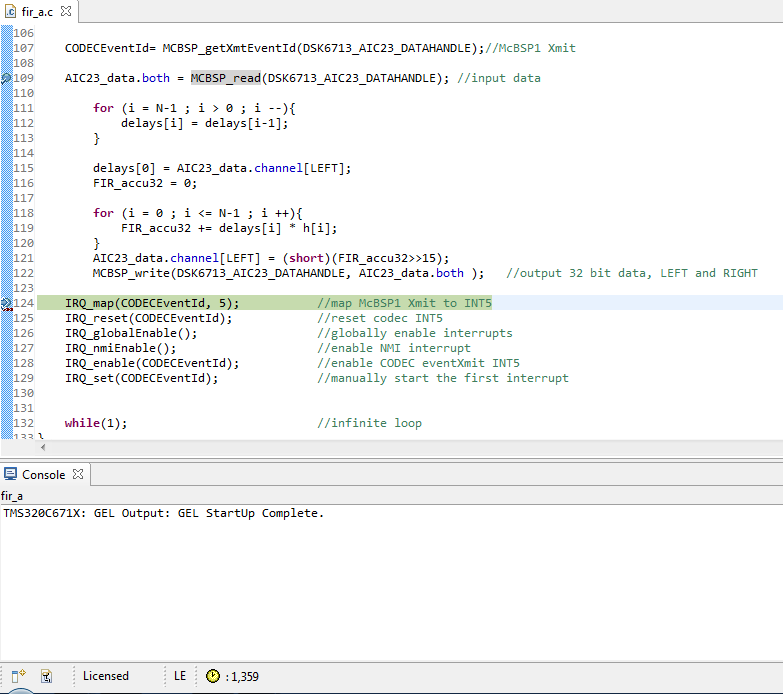
\includegraphics[width=0.9\linewidth]{Bilder/Attachment_D_Profiling}
	\caption{Durchführen des Profilings der FIR-ISR}
	\label{fig:Attachment_D_Profiling}
\end{figure}

\noindent Die maximal erlaubte Abtastfrequenz für dieses FIR-Filter, sodass der nächste Abtastwert noch korrekt eingelesen wird und kein Aliasing entsteht, berechnet sich folgendermaßen:\\

\begin{alignat}{1}
t_{Takt} &= \frac{1}{225Mhz} = 4.5ns \\
t_{ISR}  &= 1359 \cdot 4.5ns = 6.04\mu s \\
\rightarrow f_{max} &= \frac{1}{t_{ISR}} = 165 kHz
\end{alignat}

\clearpage

\subsection{E Tiefpasstransformation mit $h_{TP} \rightarrow h_{HP}$ (Substitution: z = -z)}
\noindent

\clearpage
\subsection{F Weichenfilter Amplitudengang Hoch- und Tiefpass}
\noindent \noindent Alle Projekteinstellungen sowie -konfigurationen wurden nach Laboranleitung durchgeführt. \\
\noindent Folgende Änderungen wurden durch uns in fir\_b.c ergänzt: \\
\lstinputlisting[style=c, caption={fir\_b.c C-File Auszug - Weichenfilter}, label={lst:fir_b_ISRHPTP}]{Code/fir_b.c}

\clearpage

\noindent Nach der Implementierung wurde eine Messung mit einem Frequenzsweep von 4kHz durchgeführt:

\begin{figure}[h]
	\centering
	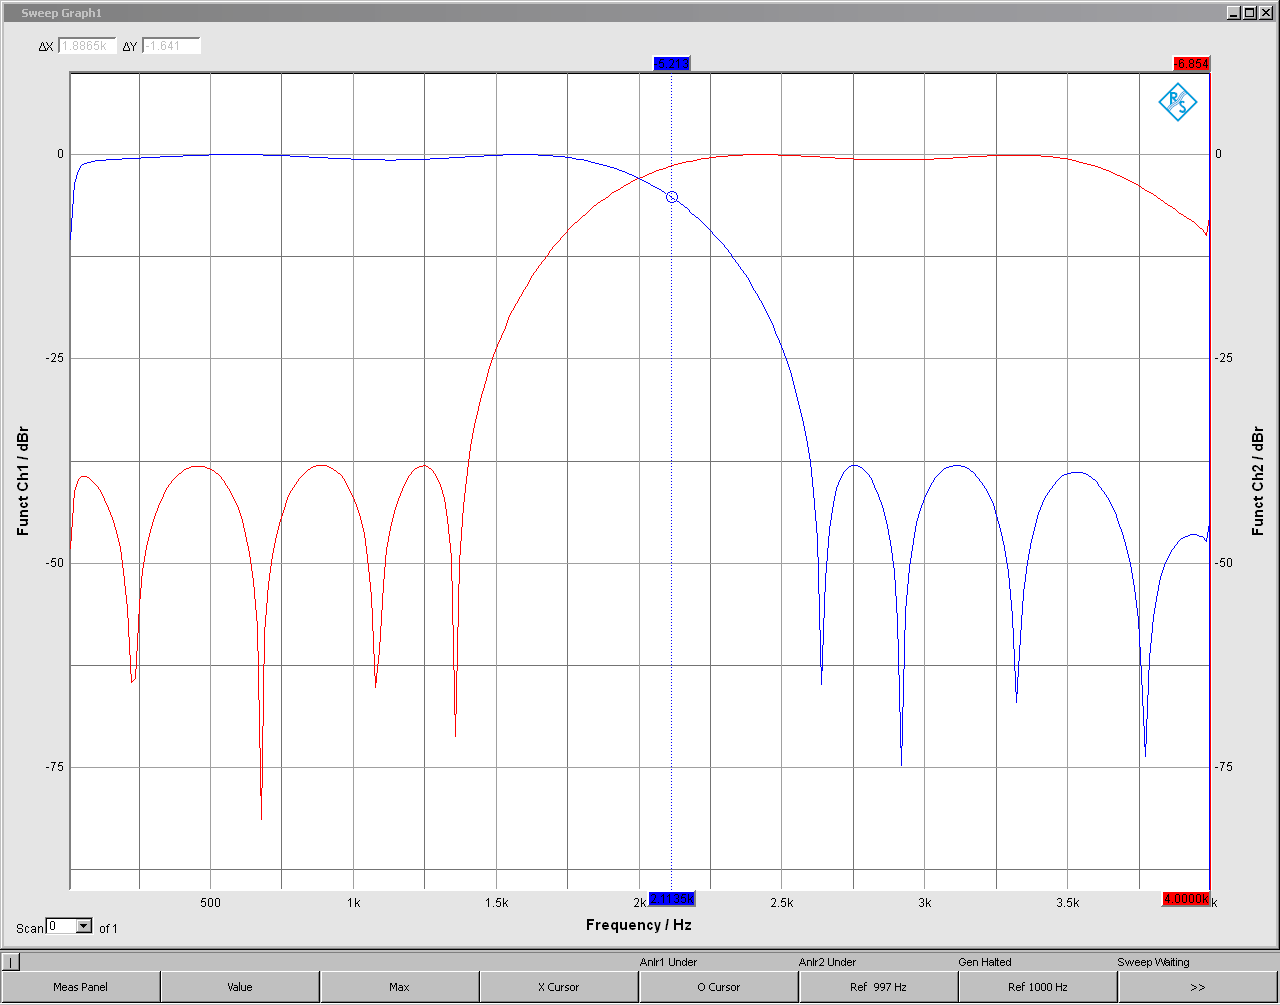
\includegraphics[width=1\linewidth]{Bilder/Attachment_F_HPTP}
	\caption{Messung: Frequenzgang des Weichenfilters mit einem 4kHz Frequenzsweep}
	\label{fig:Attachment_F_HPTP}
\end{figure}

\noindent Die beiden Amplitudengänge entsprechen unseren Erwartungen. Der Hochpass ist der gespiegelte Verlauf des Tiefpasses. Beide Sperrbereiche zeigen die gleiche Ripple-Charakteristik und Sperrdämpfung.
Im Durchlassbereich ist dies nicht so (siehe Abknicken des Durchlassbereiches des Hochpasses ab 3.5kHz),da ab 3.5kHz der Amplitudengang des DSK-Boards Einfluss nimmt. \\
\noindent Zur Programmierung der MAC-Schleife: \\
\noindent Als Grundlage diente die MAC-Schleife des FIR-Tiefpassfilters. Alle benötigten Elemente und Variablen wurden einmal für die Berechnung des FIR-Tiefpasses sowie einmal für die Berechnung des FIR-Hochpasses angelegt. Die Multiply-Accumulate-Operation für den Tiefpass blieb erhalten, lediglich eine zweite Zeile für die Multiply-Accumulate-Operation des Hochpasses wurde innerhalb dieser Schleife hinzugefügt.

\clearpage

\subsection{G Tiefpasstransformation mit $h_{TP} \rightarrow h_{HP}$ (Änderung des mittleren Koeffizienten)}
\noindent Nun sollte nur das FIR-Tiefpassfilter gemessen werden. Dem mittlere Koeffizienten (Anzahl d. Koeffizienten muss folglich ungerade sein) wurde der Wert 32767 im Watch-Window des CCS subtrahiert.\\
Folgende Abbildung zeigt die Messung mit einem Frequenzsweep von 4kHz des Analyzers:\\

\begin{figure}[h]
\centering
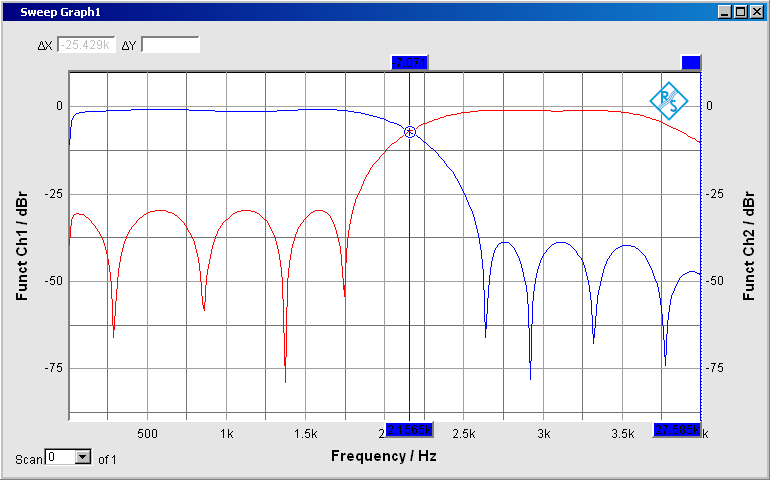
\includegraphics[width=0.7\linewidth]{Bilder/letzteAufgabe}
\caption{}
\label{fig:letzteAufgabe}
\end{figure}

 
